% !TEX root = thesis.tex

\chapter{Data analysis}
\label{cha:data_analysis}
The datasets generated with our program allow to perform some measurement regarding the use of scholarly works in the English Wikipedia.

\section{Wikipedia sections overview}
Before analyzing the behavior of the scholarly citations appearing in Wikipedia, we present a brief overview of the sections appearing in the articles.

\begin{figure}[h]
\centering
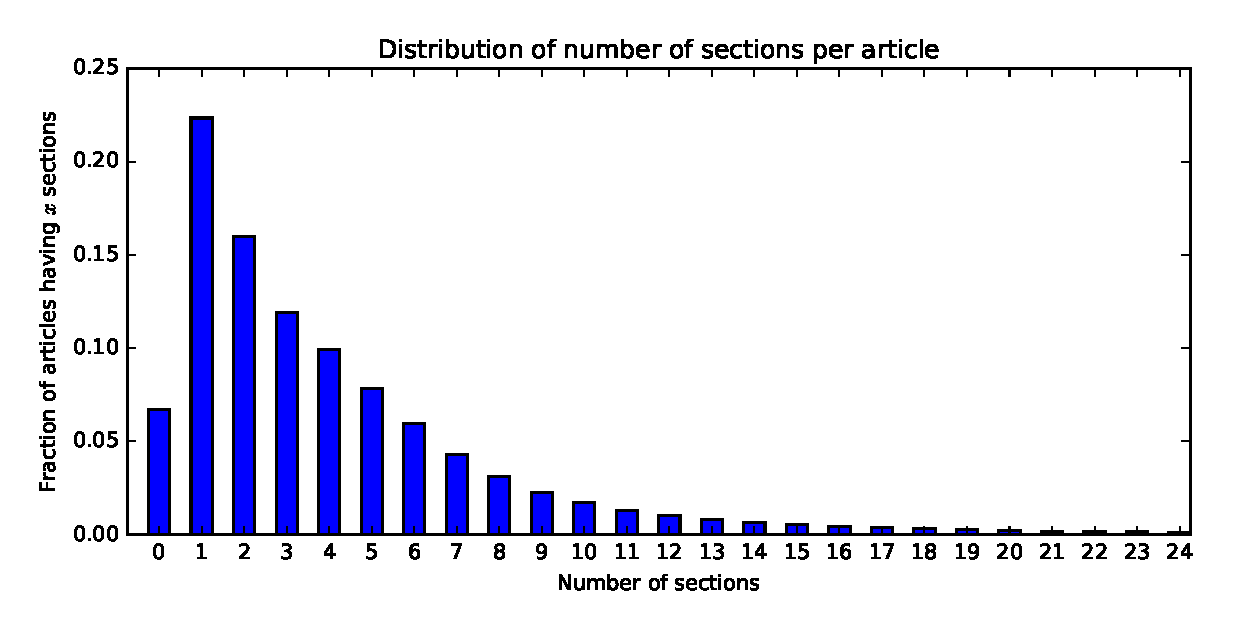
\includegraphics[keepaspectratio=true, width=\textwidth]{assets/section_counts_last_pdf}
\caption{Distribution of the number of sections per article found in the English Wikipedia at the 1st of September 2015.
Each bar represent the fraciton of articles have $x$ sections.}
\label{fig:section_counts_last_pdf}
\end{figure}

Fig.~\ref{fig:section_counts_last_pdf} show the distribution of the number of sections in Wikipedia articles at the time of the snapshot (September 1st, 2015).
The result is somewhat expected from the perspective of a Wikipedia reader: the probability of having $x$ number of sections in an article decreases with the number of sections considered.
However it is interesting to see that the distribution peaks at $x = 1$ number of sections and not at $x = 0$.

To justify this fact a further investigation is required.
However, we hypothesize that articles with less that 2 sections are usually stubs, and that they contains a ``references'' or an ``external links'' sections with the source of information used to create the article.

\begin{figure}[h]
\centering
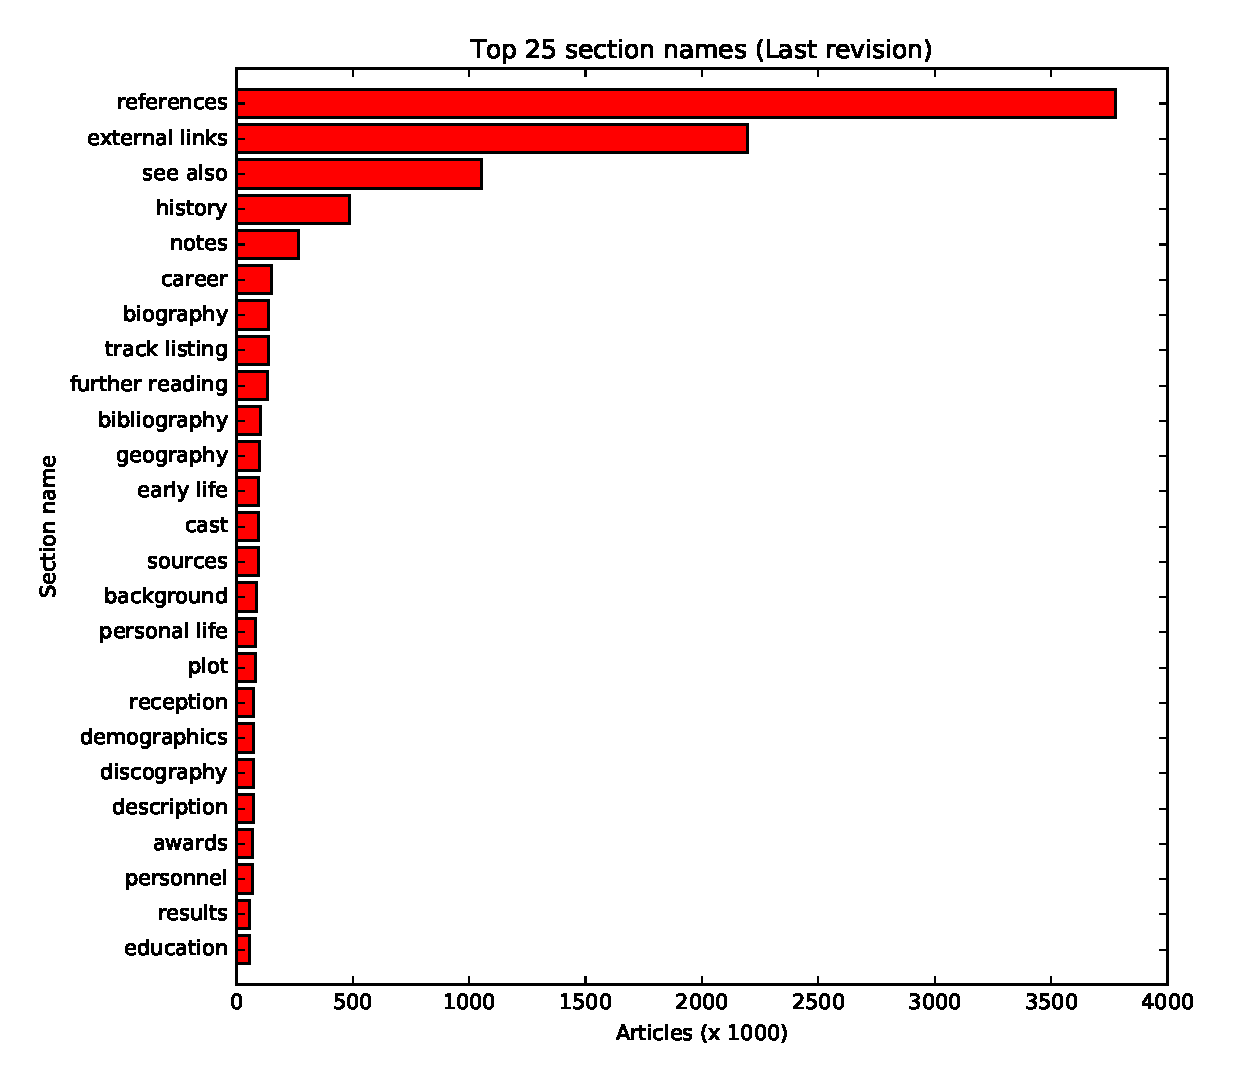
\includegraphics[keepaspectratio=true, width=\textwidth]{assets/section_names_last_top_25}
\caption{Ranking of the top 25 section names found in the English Wikipedia at the 1st of September 2015.
Each bar represent the number of articles where the section appears.}
\label{fig:section_names_last_top_25}
\end{figure}

It is also interesting to analyze which are the most common section names used.
The result is shown in Figure~\ref{fig:section_names_last_top_25}\todo{this should probably be a table}.
The most common section used is ``references''.
According to Wikipedia guidelines, this section is intended to contain citations, footnotes and general references.
Therefore it is expected that it appears in the first position of the ranking.
``External links'' usually contains links to the original material described in the article, while in ``see also'' there are usually interlinks to related articles, hence their popularity.

It is also expected to see that topics like ``career'' and ``biography'' appear together, because articles about persons usually include both of them.


\section{Papers in Wikipedia}
This section analyzes the use of papers in wikipedia.

\subsection{Incoming citations distribution}
The distribution of scholarly citations has been studied many times by the scientific community.
The problem is to understand the law that describes the \emph{distribution of citations} of papers, namely the distribution of the number of papers $N(x)$ that have been cited $x$ times.
Redner~\cite{Redner1998} suggested that this distribution has a large-$x$ power law decay $N(x) \sim x^{-\alpha}$.

\begin{figure}[h]
\centering
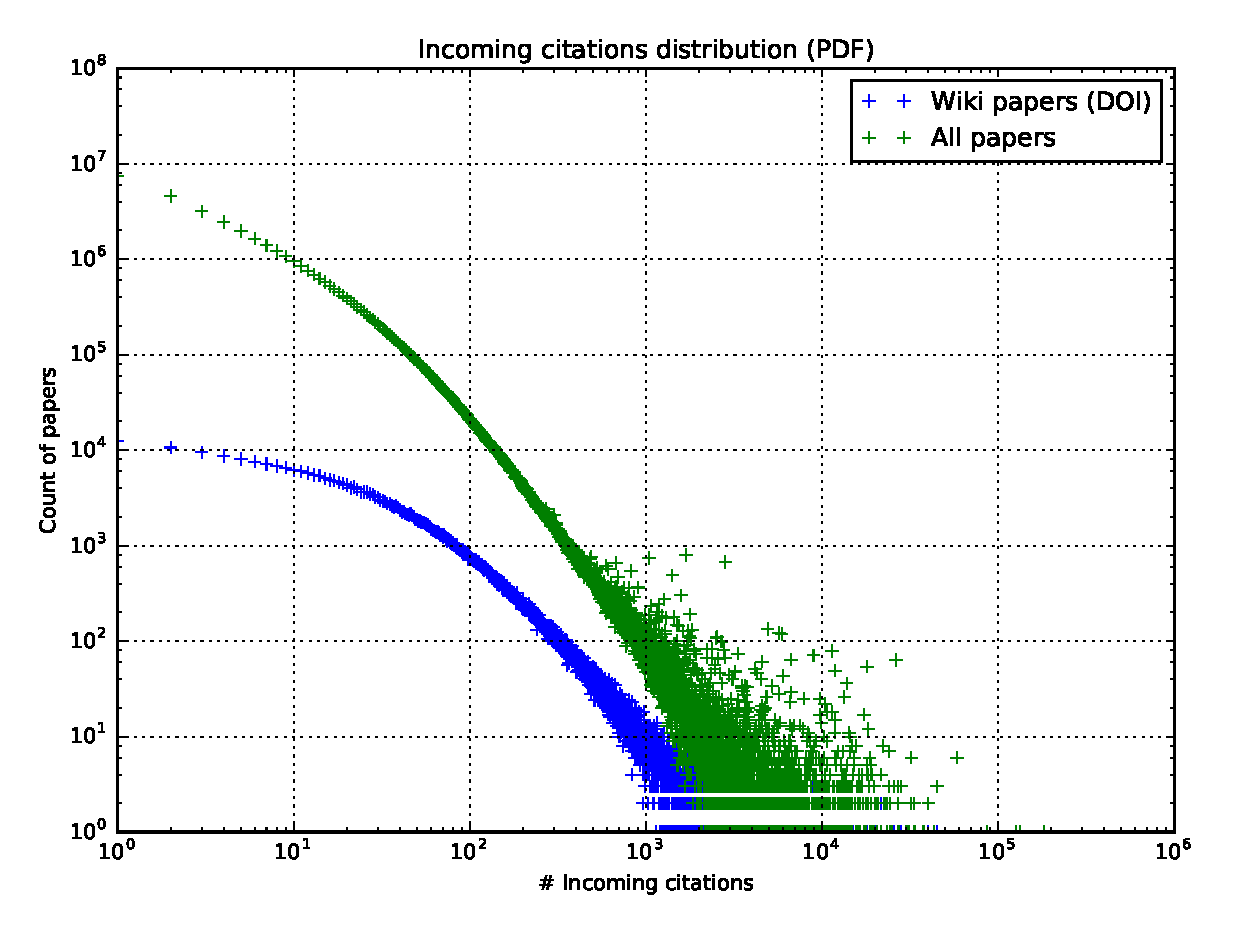
\includegraphics[keepaspectratio=true, width=\textwidth]{assets/incoming_citations_distribution_pdf}
\caption{Incoming citations distribution of papers appearing in the \ac{MAG} datasets and the ones appearing only in English Wikipedia, on a log-log scale.
On the ordinate, the number of papers having exactly $x$ incoming references, globally.}
\label{fig:incoming_citations_distribution_pdf}
\end{figure}

Fig.~\ref{fig:incoming_citations_distribution_pdf} compares the distribution of citations of all the papers known to the MAG (circa 120 millions) and the ones whose \ac{DOI} appears in Wikipedia (circa 389 thousands).
The number of incoming citation for a paper is determined using the \ac{MAG} dataset.
Notice that the only identifier available in the \ac{MAG} is the \ac{DOI}, hence only the papers found in Wikipedia which have a \ac{DOI} are considered.
This accounts for the 28\% of the identifiers found.
Furthermore, from this set of papers we removed the ones that appears to be ``non-valid'' in the \ac{MAG} dataset, namely the ones that have more than one \ac{DOI}.
The amount of papers considered at the end is the 17\% of the identifiers found in Wikipedia.

This graph alone does not give much information.
It is more interesting to analyze the \ac{ccdf} of the two series.
The \ac{ccdf}, or \emph{tail distribution}, expresses the percentage of papers $\bar{F}(x)$ that have at least $x$ citations.

\begin{figure}[h]
\centering
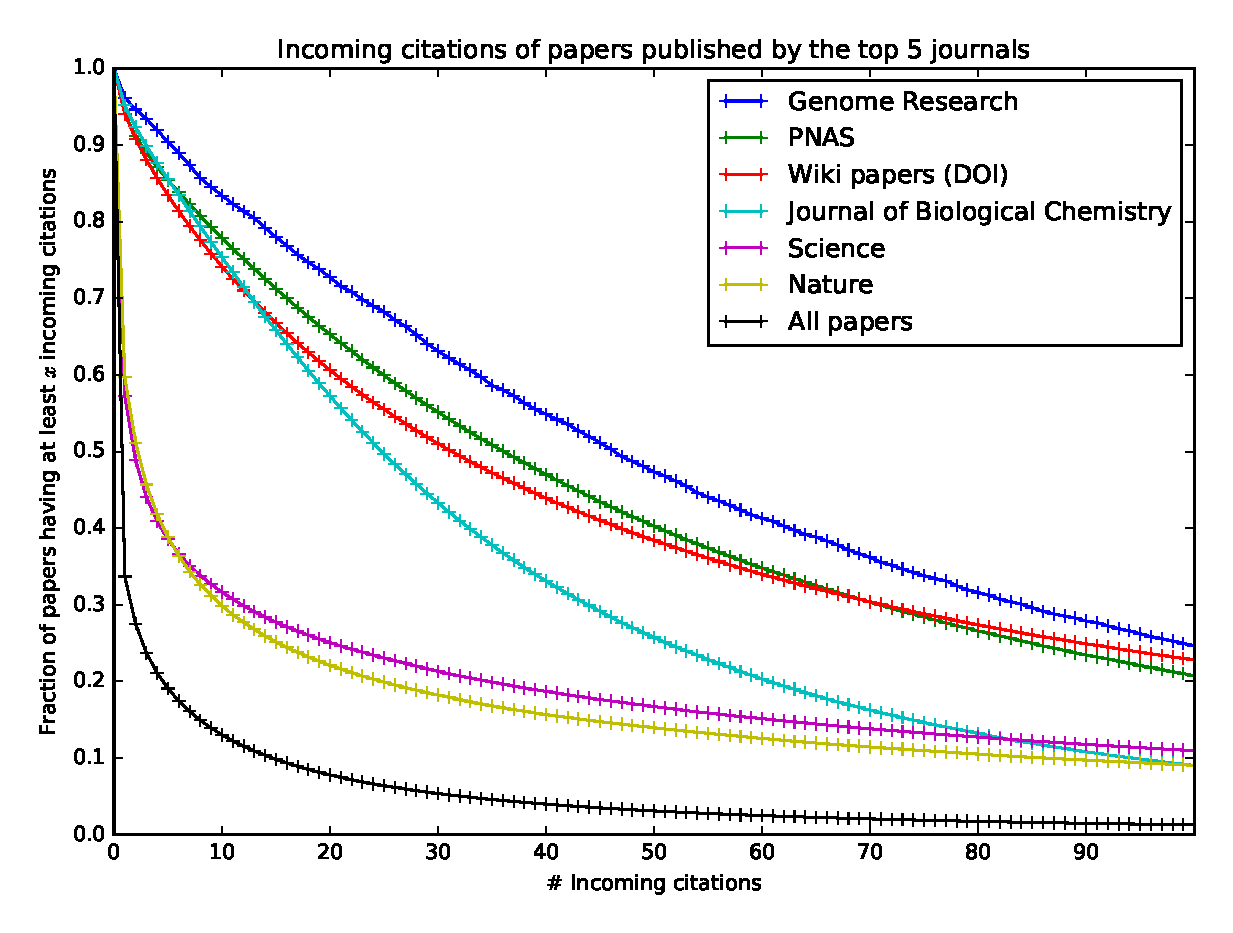
\includegraphics[keepaspectratio=true, width=\textwidth]{assets/incoming_citations_distribution_ccdf}
\caption{Tail distribution of the incoming citations of papers appearing in Wikipidia compared with the ones appearing in the top 5 cited journals.
On the ordinate, the fraction of papers having at least $x$ incoming references.}
\label{fig:incoming_citations_distribution_ccdf}
\end{figure}

\begin{table}[]
\centering
\begin{tabular}{@{}lr@{}}
\toprule
\multicolumn{1}{c}{\textbf{Journal}} & \textbf{Wikipedia citations} \\ \midrule
PNAS                                 & 16273                        \\
Nature                               & 13403                        \\
Science                              & 11019                        \\
Journal of Biological Chemistry      & 8587                         \\
Genome Research                      & 6850                         \\ \bottomrule
\end{tabular}
\caption{Top 5 journals cited in Wikipedia articles, with the number of distinct citations in different articles.}
\label{tbl:top_cited_wikipedia_journals}
\end{table}

Figure~\ref{fig:incoming_citations_distribution_ccdf} shows the cumulative distribution of the incoming citations of papers in Wikipedia and compares it with the one of the top cited papers in Wikipedia, represented in Table~\ref{tbl:top_cited_wikipedia_journals}.
First of all, papers appearing in Wikipedia tend to have many more incoming citations with respect to a random paper taken from all the available ones.
This is expected and we would be surprise if that was not the case.
For instance, the 74\% of papers in Wikipedia have at least 10 incoming citations, while only the 13\% of papers have at least 10 incoming citations.

More useful is the comparison between the behavior of papers in Wikipedia with some of the most cited journals in Wikipedia.
The ``goodness'' of them is second only to papers that have been published in \emph{Genome Research} or \emph{PNAS}, while they outclass journals like \emph{Science} and \emph{Nature}.

However, we have to keep in mind that Wikipedia contains a selection of papers, and thus it is just a confirmation that the ones that appear already had an impact on the scientific community.

The fact that more than the 40\% of papers published by \emph{Science} or \emph{Nature} have zero incoming citations in the scientific community was not expected.
We want to exclude the hypothesis that they did not have much time to get an impact on the community.

\begin{figure}[h]
\centering
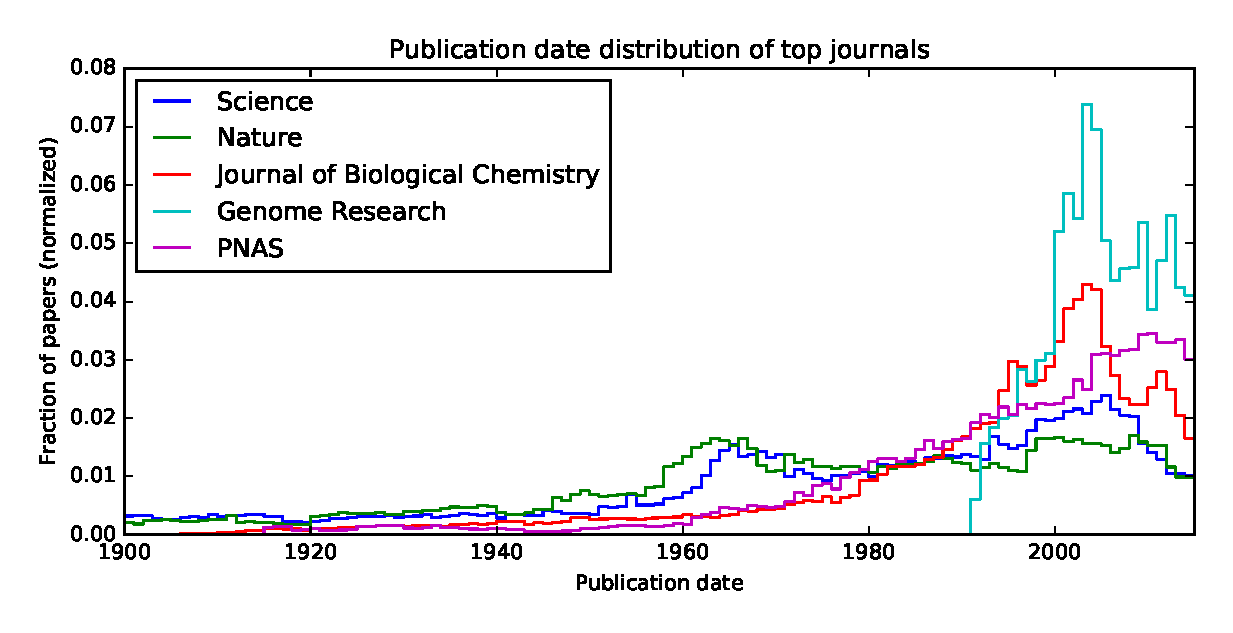
\includegraphics[keepaspectratio=true, width=\textwidth]{assets/publication_date_distribution_journals}
\caption{Publication date distribution of the top 5 journals cited in Wikipedia, starting from the 1900.
On the ordinate, the fraction of papers published in each year.}
\label{fig:publication_date_distribution_journals}
\end{figure}

\begin{figure}[h]
\centering
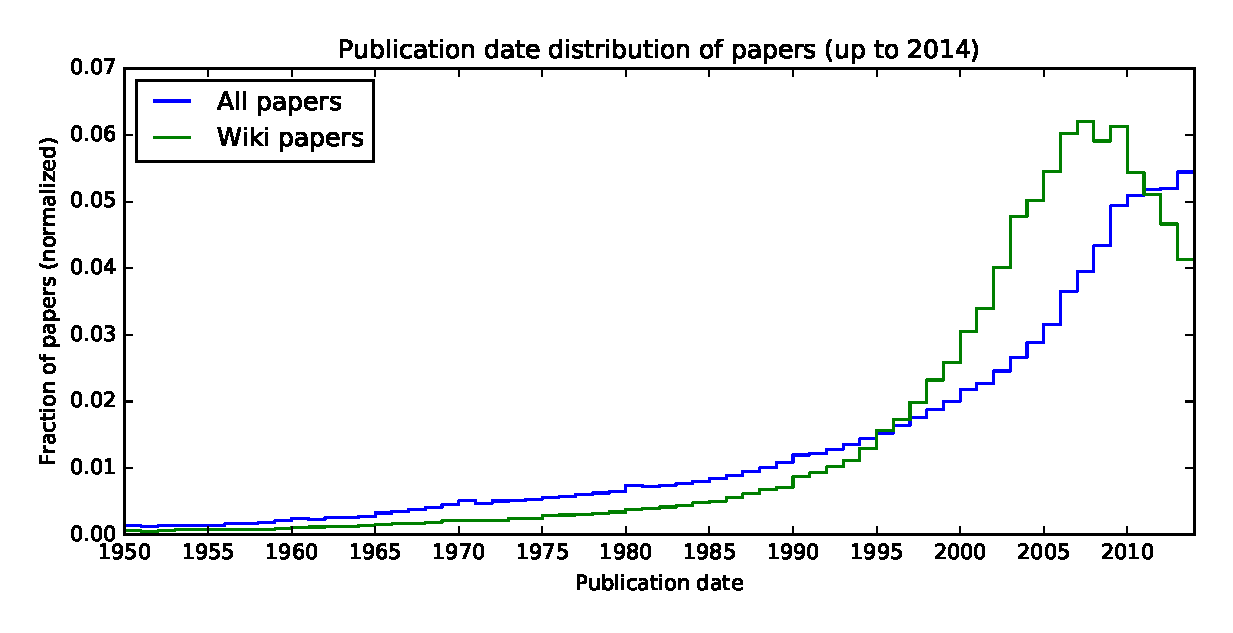
\includegraphics[keepaspectratio=true, width=\textwidth]{assets/publication_date_pdf}
\caption{Publication date distribution of all the known papers the ones found in Wikipedia in the last 60 years, up to the 2014.
On the ordinate, the fraction of papers published in each year.
}
\label{fig:publication_date_pdf}
\end{figure}

The graph in Figure~\ref{fig:publication_date_distribution_journals} shows the publication date distribution of the top 5 journals cited in Wikipedia.
We can see that many of the papers published in the \emph{Genome Research} are not older than 20 years, yet most of them have a good number of citations.
Instead, papers in \emph{Nature} and \emph{Science} are older but still they do not get as many citations.

Figure~\ref{fig:publication_date_pdf} compares the same distribution for papers appearing in Wikipedia with all the known ones.
Wikipedia articles tend to cite papers which are released in the last few years.
This is expected because that the number of papers published grows each year and because many works are replicated and extended by other authors and only the newer ones tend to be cited.

From the plot we can also see that the number of papers published increases each year.
In 1961, Price~\cite{Price1961} studied the growth of scientific publications covering the period from about 1650 to 1950.
The data indicated a growth rate of about 5.6\% per year and a doubling time of 13 years.

The study of this matter has then been propose again by many, showing that the growth varies depending on the dataset used and analyzing different period of times.
For instance, Larsen et al.~\cite{Larsen2010} in the 2010 studied the growth using different datasets and limited to the time period between the 1907 and the 2007.
They showed that there are many other factors that determine the growth of publications that should be considered.

We have reproduced the result of Larsen et al.\ using the linear regression method, and we have obtained comparable results: the overall growth rate we have found is about 3,98\% and a doubling time of 17,4 years.
Fig.~\ref{fig:publication_date_regression} compares the actual growth with the one we have derived.

\begin{figure}[h]
\centering
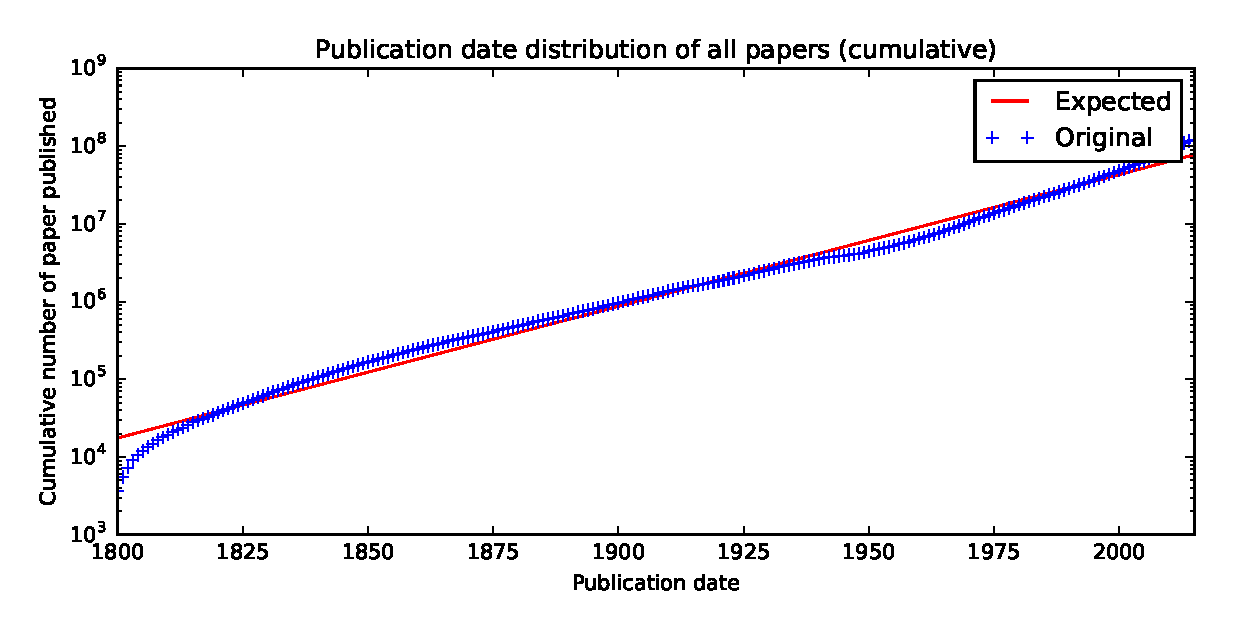
\includegraphics[keepaspectratio=true, width=\textwidth]{assets/publication_date_regression}
\caption{Publication date count for all the papers appearing in the \ac{MAG} dataset and the estimate obtained with the linear regression method.}
\label{fig:publication_date_regression}
\end{figure}

\subsection{Age of identifiers at first appearance}
Another interesting information to analyze is the age of the papers when they first appear in Wikipedia.
Fig.~\ref{fig:age_of_papers_at_first_appearance_pdf} shows the distribution of the age of papers when they are referenced on Wikipedia for the first time.
We do not expect to see negative values, because this would mean that an identifier appears in Wikipedia before the paper is published.
In practice this happens because the \ac{MAG} dataset is not 100\% accurate, and some publication dates may contain errors.
We have investigated this problem, and it seems to be caused by how Microsoft extracts the publication date of a paper.
It appears that if a paper is published online on a certain date, and it is also released after in a journal, Microsoft consider the date of the journal the publication date.
However, only the 3,12\% of the \acp{DOI} extracted have a negative age, so the effect of this error is arguably marginal, as we can see from Figure~\ref{fig:age_of_papers_at_first_appearance_cdf}.
This plot shows cumulative distribution of the series, namely what is the percentage $F(x)$ of paper identifiers which are inserted in Wikipedia at most $x$ days after their publication.

It is interesting to see that many \acp{DOI} have been inserted in Wikipedia a few days after their publication (Figure~\ref{fig:age_of_papers_at_first_appearance_pdf_near0}).
We have analyzed some of these cases, and it appears that that some authors insert the identifier of their paper in a Wikipedia article as soon as it has been published.
However, these cases do not play a major role in the overall distribution since they account for just the 0,49\% of papers inserted.



\begin{figure}[h]
    \centering
    \begin{subfigure}{1\textwidth}
        \centering
        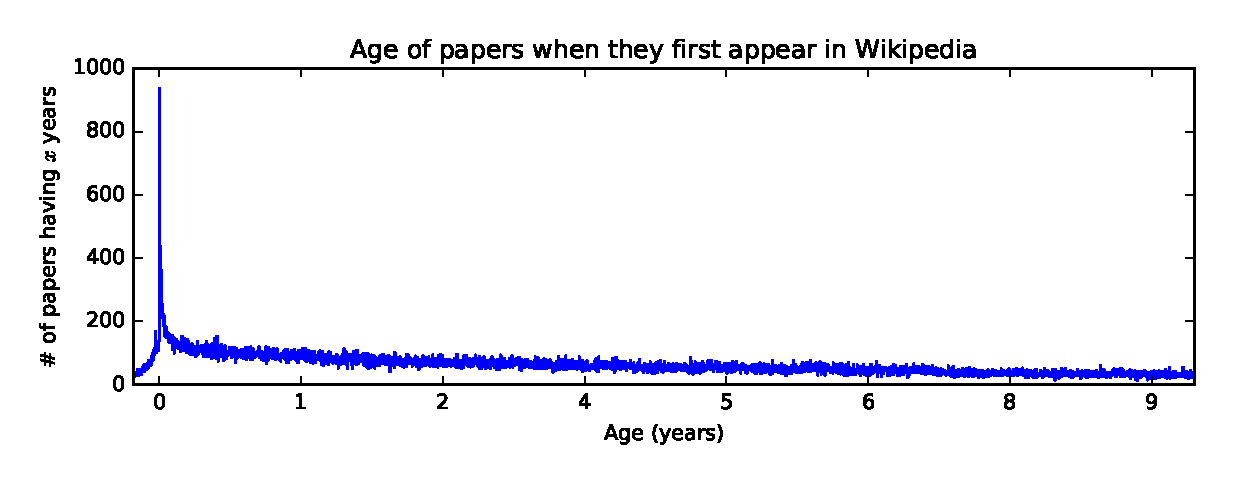
\includegraphics[keepaspectratio=true, width=\linewidth]{assets/age_of_papers_at_first_appearance_pdf}
        \caption{Cumulative distribution of the age of papers when they appear for the first time on Wikipedia.}
\label{fig:age_of_papers_at_first_appearance_pdf}
    \end{subfigure}
    \begin{subfigure}{1\textwidth}
        \centering
        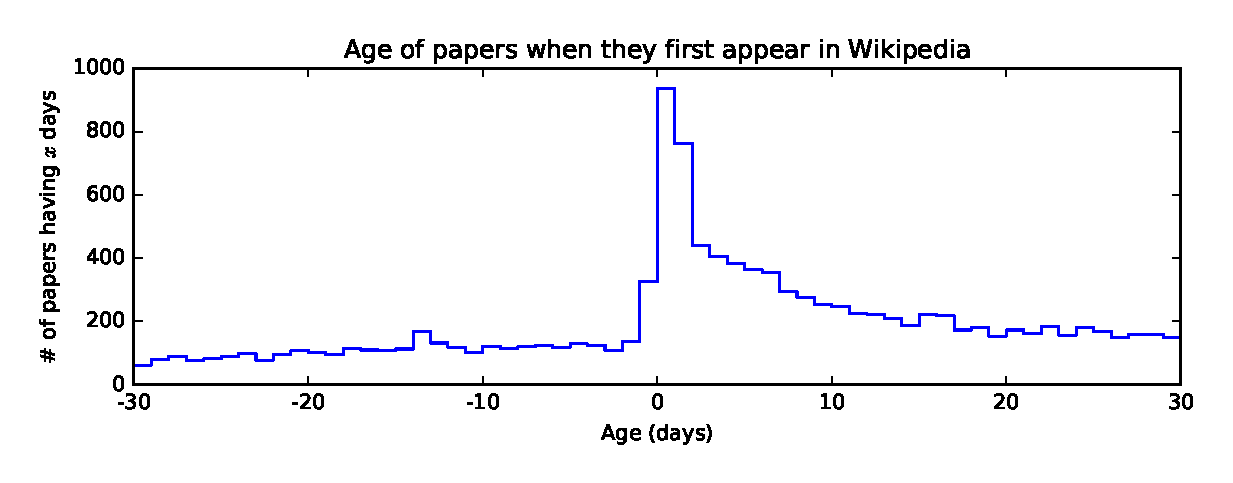
\includegraphics[keepaspectratio=true, width=\linewidth]{assets/age_of_papers_at_first_appearance_pdf_near0}
        \caption{Distribution of the age of papers when their DOI appear for the first time on Wikipedia, specifically between $[-30, 30]$ days.}
\label{fig:age_of_papers_at_first_appearance_pdf_near0}
    \end{subfigure}
    \begin{subfigure}{1\textwidth}
        \centering
        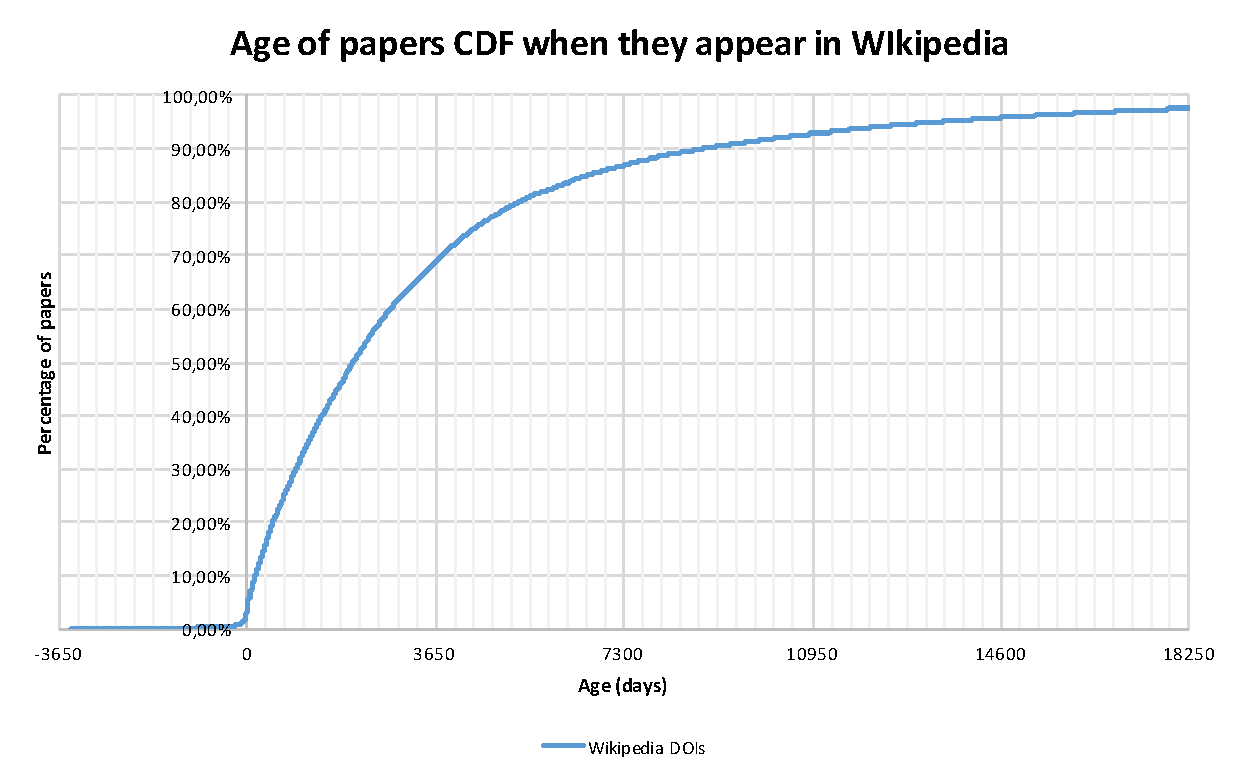
\includegraphics[keepaspectratio=true, width=\linewidth]{assets/age_of_papers_at_first_appearance_cdf}
        \caption{Cumulative distribution of the age of papers when they appear for the first time on Wikipedia.}
\label{fig:age_of_papers_at_first_appearance_cdf}
    \end{subfigure}
\end{figure}

\subsection{Lifetime of irrelevant citations inside an article}
It is interesting to analyze how long academic citations live inside a page.
In particular, the focus of this sections is on publication identifiers which have been inserted in a page and then removed for some reason, most probably because of irrelevance.
The rationale behind this choice is to analyze how long does it take for a Wikipedia contributor to discover and remove an irrelevant identifier appearing in an article.

We define the notion of irrelevance as follows: an identifier is considered \emph{irrelevant} for a Wikipedia article if it appeared on that article in the past but it does no more appear in that page at the time of the snapshot being taken, in our case the 1st of September 2015.

The lifetime of irrelevant identifiers found in different pages is depicted in the left column of Figure~\ref{fig:irrelevant_identifiers_and_dois}, by the meaning of plots displaying the cumulative distribution function.
The ordinate describe how many identifiers in different pages lived at most $x$ time units (e.g.\ years, months or days).
In another way, the graphs show how long did it take for the Wikipedians to remove the irrelevant identifiers from the articles where they appear.
Each series describe the behavior of a certain type of identifier (i.e.\ \ac{ISBN}, \ac{DOI}, \ac{PMID} or \emph{arXiv})
All the curves starts with a steep climb in the first period of time.
Indeed more than the 60\% of irrelevant \ac{ISBN} and \ac{DOI} ``lived'' in articles for less than one year.
Something more worth of notice is that 35\% of \acp{DOI} ``lived'' less than one month, and more than the 20\% less then one day.

However, it may also be the case that many identifiers are removed almost immediately because they are typos made by a contributor while he was editing the page.

We have a way to distinguish \acp{DOI} which are valid (i.e.\ that refer to an existing object) from the ones that are not.
We first search for the DOI in the MAG corpus: if it exists then it is valid, otherwise we query directly the DOI authority using the available APIs\footnote{\url{http://www.doi.org/factsheets/DOIProxy.html}}.


Figure~\ref{fig:irrelevant_identifiers_count} shows the number of \acp{DOI} appearances that are generated by valid and invalid DOIs.
We observe that just the 4\% of them are due to an unrecognized identifier, most probably a typo.
The right column of Figure~\ref{fig:irrelevant_identifiers_and_dois} shows how long DOIs lived inside Wikipedia articles, along with the ones that are not recognized.
We observe, as expected, that the latter do not play a major role in the distribution.
This fact reject the hypothesis that a good part of irrelevant DOIs are removed almost immediately because they are typos made by editors.

Considering the fact that more than the 20\% of irrelevant \acp{ISBN} and \acp{DOI} are removed within the first day, we conclude that the effort made by Wikipedians to remove irrelevant references inside the articles is both remarkable and effective.

\begin{figure}[h]
    \centering
    \begin{subfigure}{.5\textwidth}
        \centering
        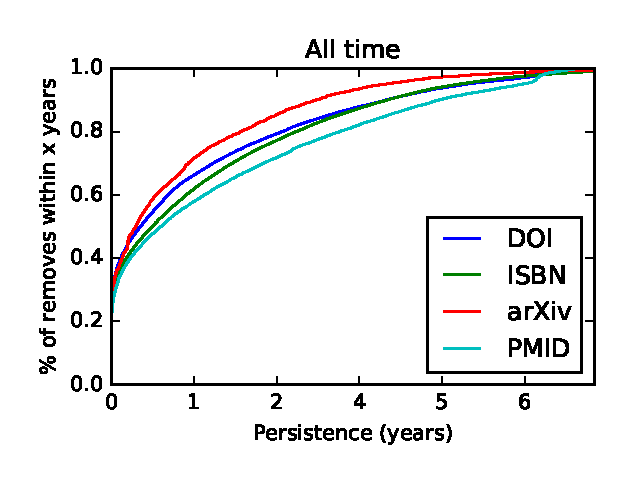
\includegraphics[keepaspectratio=true, width=1\linewidth]{assets/irrelevant_identifiers_persistence_cdf_max}
\label{fig:irrelevant_identifiers_persistence_cdf_max}
    \end{subfigure}%
    \begin{subfigure}{.5\textwidth}
        \centering
        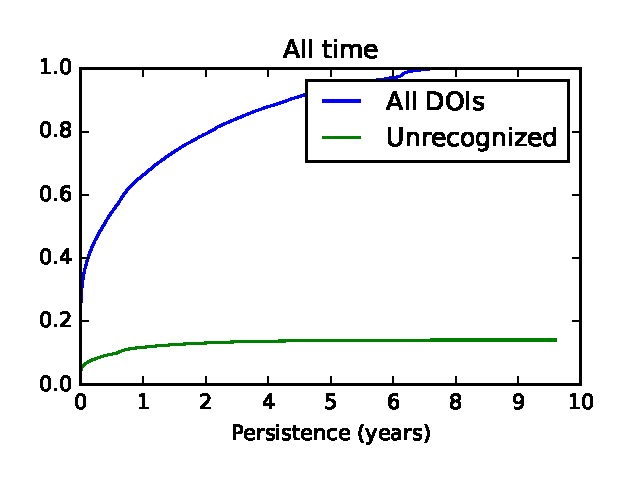
\includegraphics[keepaspectratio=true, width=1\linewidth]{assets/irrelevant_doi_persistence_cdf_max}
\label{fig:irrelevant_doi_persistence_cdf_max}
    \end{subfigure}

    \begin{subfigure}{.5\textwidth}
        \centering
        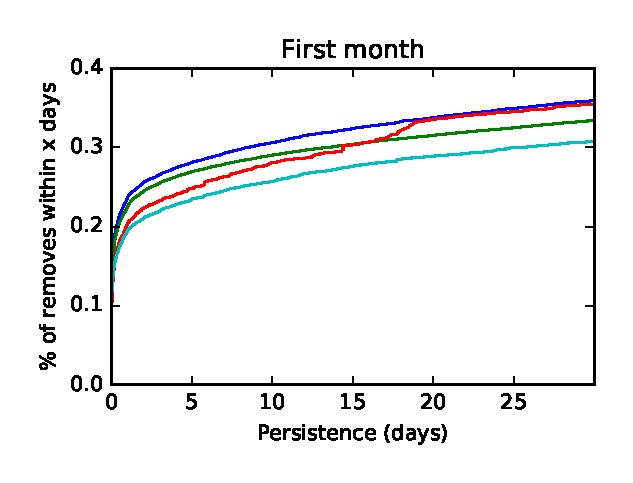
\includegraphics[keepaspectratio=true, width=1\linewidth]{assets/irrelevant_identifiers_persistence_cdf_1month}
\label{fig:irrelevant_identifiers_persistence_cdf_1month}
    \end{subfigure}%
    \begin{subfigure}{.5\textwidth}
        \centering
        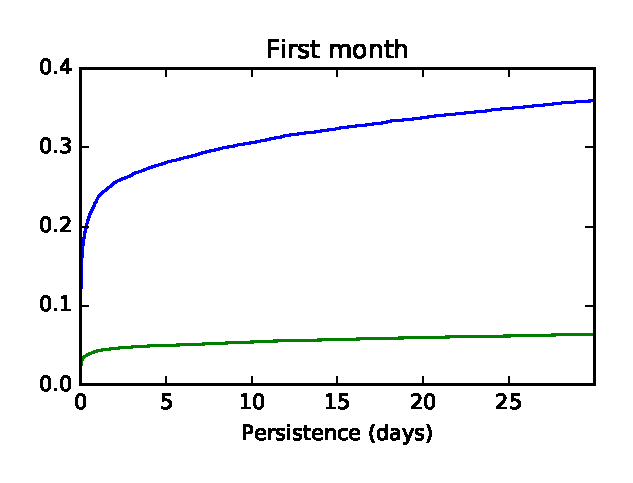
\includegraphics[keepaspectratio=true, width=1\linewidth]{assets/irrelevant_doi_persistence_cdf_1month}
\label{fig:irrelevant_doi_persistence_cdf_1month}
    \end{subfigure}

    \begin{subfigure}{.5\textwidth}
        \centering
        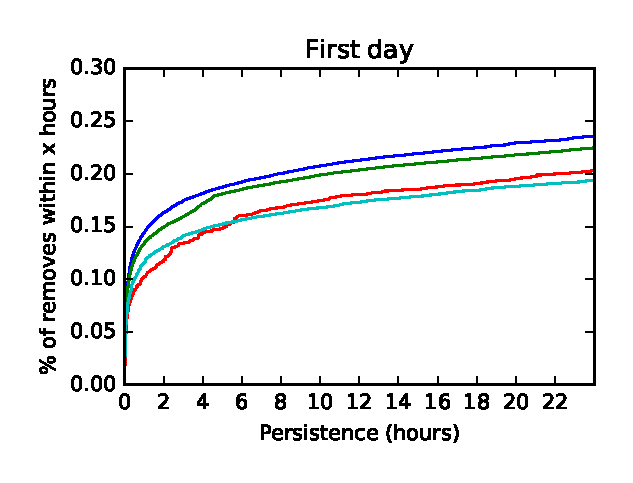
\includegraphics[keepaspectratio=true, width=1\linewidth]{assets/irrelevant_identifiers_persistence_cdf_1day}
\label{fig:irrelevant_identifiers_persistence_cdf_1day}
    \end{subfigure}%
    \begin{subfigure}{.5\textwidth}
        \centering
        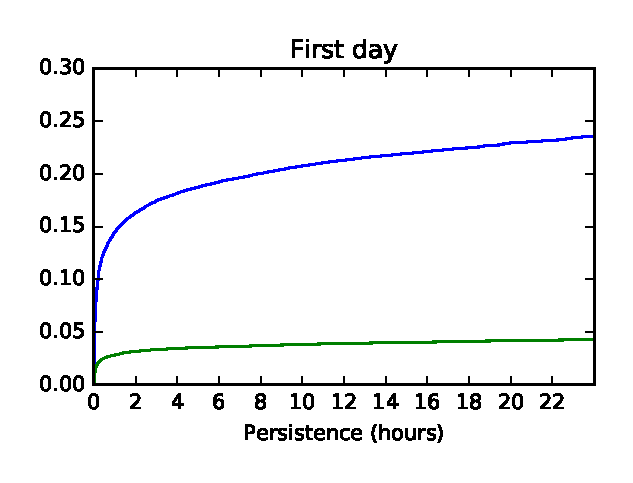
\includegraphics[keepaspectratio=true, width=1\linewidth]{assets/irrelevant_doi_persistence_cdf_1day}
\label{fig:irrelevant_doi_persistence_cdf_1day}
    \end{subfigure}
    \caption{On the left column: distribution of the time required to remove irrelevant identifiers, with a detailed view of the first month and the first day.
    On the right column: distribution of the time required to remove irrelevant DOIs, along with the number of unrecognized DOIs.
    The y-axis describes the ratio of identifier removed in different Wikipedia articles within $x$ time units.}
\label{fig:irrelevant_identifiers_and_dois}
\end{figure}

\begin{figure}[h]
    \centering
    \begin{subfigure}{.5\textwidth}
        \centering
        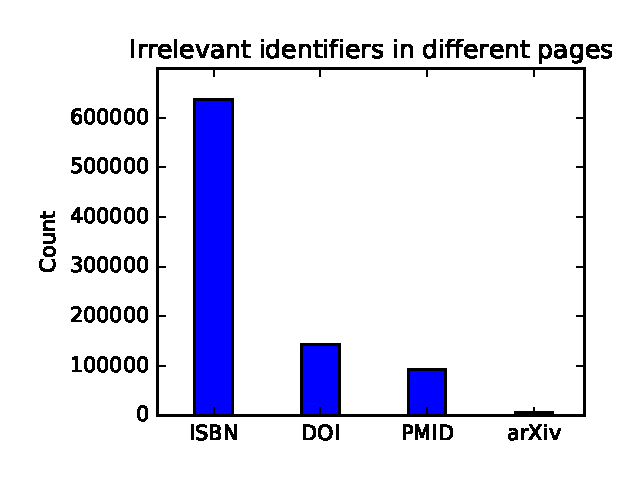
\includegraphics[keepaspectratio=true, width=\textwidth]{assets/irrelevant_identifiers_count_by_type}
    \end{subfigure}%
    \begin{subfigure}{.5\textwidth}
        \centering
        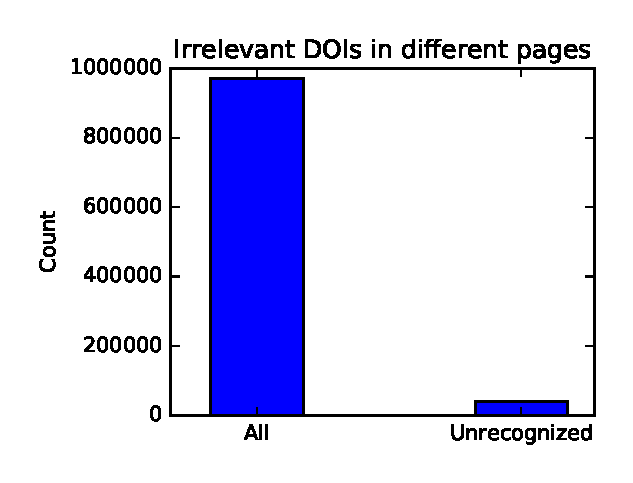
\includegraphics[keepaspectratio=true, width=\textwidth]{assets/irrelevant_doi_count_by_validity}
    \end{subfigure}
    \caption{On the left side: number of irrelevant identifiers appearances in different Wikipedia articles.
    On the right side: the number of appearances of DOIs not recognized by the authority along with the total number of DOI appearances.}
\label{fig:irrelevant_identifiers_count}
\end{figure}

%A word of caution: we assume that if an identifier has been removed from a page and it is not present in the last revision at the time of the dump, then its appearance in the page is not relevant.
